\section{Cell homogenisation and equivalence theory}

Now, armed with the language of collision probabilities, we return to slowing down. But this time, we will assert that there is heterogeneity, namely, a cylindrical fuel region and a surrounding moderator region.

We will use the following notation:
\begin{itemize}
    \item f: fuel
    \item m: moderator
    \item 0: absorber nuclide in fuel
    \item 1: moderator nuclide in fuel
    \item 2: moderator nuclide in the moderator
\end{itemize}
In a given region and for a given nuclide, our scattering source will look like:
\begin{equation*}
    I_i(\phi_z) \equiv \int^{E/\alpha_i}_{E}\frac{\mathrm{d}E'}{(1-\alpha_i)E'}\Sigma_{\mathrm{s},i}\phi_z(E')\;\mathrm{,}
\end{equation*}
where $i$ refers to the nuclide, $z$ refers to the zone.

We will make some additional notation:
\begin{itemize}
    \item $P_{\mathrm{f}\rightarrow\mathrm{m}}(E)$: probability for a neutron born in the moderator with energy $E$ to enter the fuel and collide there for the first time.
    \item $P_{\mathrm{m}\rightarrow\mathrm{f}}(E)$: the same, but in the other direction
    \item $V_\mathrm{m}$, $V_\mathrm{f}$: the volumes of the moderator and fuel.
    \item $\phi_\mathrm{m}$, $\phi_\mathrm{f}$: zone average fluxes in the moderator and fuel.
\end{itemize}

Given this, in our heterogeneous system, the neutron balance equation in the fuel looks like:
\begin{equation*}
    V_\mathrm{f}\phi_\mathrm{f}(E)\Sigma_\mathrm{t,f}(E) = V_\mathrm{f}(1-P_{\mathrm{f}\rightarrow\mathrm{m}}(E))\times(I_0(\phi_\mathrm{f}) + I_1(\phi_\mathrm{f})) + V_\mathrm{m}P_{\mathrm{m}\rightarrow\mathrm{f}}(E)I_2(\phi_\mathrm{m})\;\mathrm{.}
\end{equation*}
For the moment, we will assume that \textbf{if a neutron escapes the fuel, it will collide in the moderator with 100\% certainty}. We will hence refer to $P_{\mathrm{f}\rightarrow\mathrm{m}}$ as the escape probability, $P_\mathrm{escape}$, or $P_\mathrm{esc}$. This is obviously wrong but we will correct it later.

The path forward from here is:
\begin{enumerate}
    \item Calculate $P_\mathrm{esc}$
    \item Connect $P_\mathrm{esc}$ to $P_{\mathrm{m}\rightarrow\mathrm{f}}$
    \item Solve the 2-zone slowing down equation
    \item Relax the ``isolated rod'' assumption, generalising to tight lattices
    \item Produce estimates for $\phi_\mathrm{f}(E)$ and $\phi_\mathrm{m}(E)$ to calculate cross sections
\end{enumerate}

\subsection{Estimating the escape probability}

We need to calculate the probability that a neutron leaves the fuel (given we have assumed an isolated system -- if it weren't, we would need to account for it colliding in another fuel element beyond the moderator).

For a neutron in the fuel, flying in direction $\mathbf{\Omega}$, with a distance of $s$ to the surface of the fuel, the probability of travelling that distance is $\exp{\left(-\Sigma_{\mathrm{t,f}}(E)s\right)}$. The small volume surrounding the neutron can be expressed as $(\mathbf{n}\cdot\mathbf{\Omega})\mathrm{d}S\mathrm{d}s$, where $\mathrm{d}S$ is a small surface element of the total surface, $S$, and $\mathbf{n}$ is the inward normal vector from that surface element. The geometry of this setup is shown in Fig.~\ref{fig:escape}. For a fixed direction, if we sum over all surfaces and distances to the surface, we would estimate the escape probability as:
\begin{equation*}
    P_\mathrm{esc}(E,\mathbf{\Omega}) = \frac{1}{V_\mathrm{f}}\int_{S}\mathrm{d}S\left(\mathbf{n}\cdot\mathbf{\Omega}\right)\int^l_0\mathrm{d}s \exp\left(-\Sigma_{\mathrm{t,f}}(E)s\right) = \frac{1}{\Sigma_{\mathrm{t,f}}(E)V_\mathrm{f}}\int_S\mathrm{d}S \left(\mathbf{n}\cdot\mathbf{\Omega}\right)\times\left(1-\exp\left(-\Sigma_\mathrm{t,f}(E)l\right)\right)\;\mathrm{,}
\end{equation*}
where $l$ is the chord length, or distance from one surface to another in a given direction. We also want to average over angle, so we need integrate over that as well:
\begin{equation*}
    P_\mathrm{esc}(E) = \frac{1}{4\pi}\int_{\mathbf{n}\cdot\mathbf{\Omega}>0}\mathrm{d}\Omega P_\mathrm{esc}(E,\mathbf{\Omega})= \frac{1}{4\pi\Sigma_{\mathrm{t,f}}(E)V_\mathrm{f}}\int_{\mathbf{n}\cdot\mathbf{\Omega}>0}\mathrm{d}\Omega\int_S\mathrm{d}S \left(\mathbf{n}\cdot\mathbf{\Omega}\right)\times\left(1-\exp\left(-\Sigma_\mathrm{t,f}(E)l\right)\right)\;\mathrm{.}
\end{equation*}
To resolve this integral, we need to know how the chord length, $l$, is distributed. Even if we did, the result for evaluating this integral is complicated and (at least historically) painful to evaluate. For example, for a slab of width $a$, this would produce:
\begin{equation*}
    P_\mathrm{esc}(E) = \frac{1}{\Sigma_{\mathrm{t,f}}(E)a}\left[\frac{1}{2}-E_3(\Sigma_{\mathrm{t,f}}(E)a)\right]\;\mathrm{,}
\end{equation*}
where $E_3$ is an exponential integral:
\begin{equation}
    E_3(y) = \int^\infty_1\mathrm{d}x x^{-3}\exp\left(-yx\right)\;\mathrm{.}
\end{equation}

\begin{figure}[h]
  \centering
  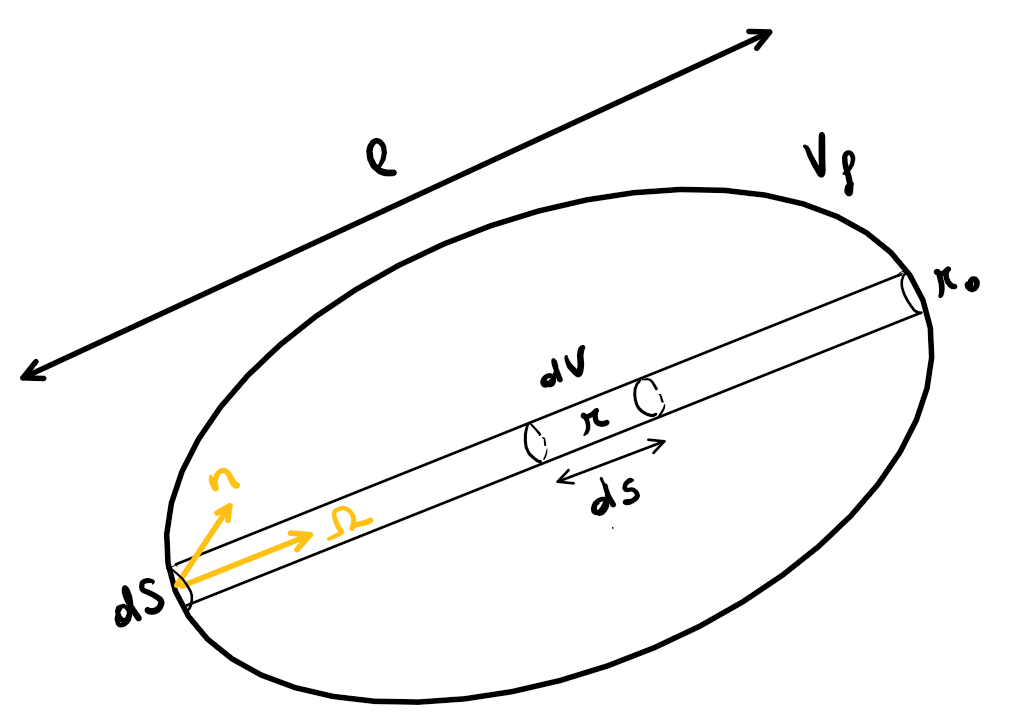
\includegraphics[scale=0.60]{./Figures/P6/escapeProb.png} 
  \caption{Geometry for estimating the escape probability.} 
  \label{fig:escape}
\end{figure}

\subsection{Wigner's rational approximation}

Generally, we can say some things about the chord length and escape probability. For a convex body, it is known (from Dirac) that the average chord length, $\bar{l}$ is simply
\begin{equation*}
    \bar{l} = \frac{4V}{A}\;\mathrm{,}
\end{equation*}
where $V$ is the volume of the region and $A$ is the surface area. We will try to obtain $P_\mathrm{esc}$ in terms of this quantity. 

From physical intuition, we can reason that as bodies become small/optically thin (or $\Sigma_\mathrm{t,f}\bar{l}\rightarrow 0$), $P_\mathrm{esc}\rightarrow~1$. We can show what happens as bodies become large, or $\Sigma_\mathrm{t,f}\bar{l}\rightarrow \infty$. In this scenario, $e^{-\Sigma_\mathrm{t,f}l}<< 1$, so, $1-e^{-\Sigma_\mathrm{t,f}l}\approx 1$. This reduces our escape probability to:
\begin{equation*}
    P_\mathrm{esc}\approx \frac{1}{4\pi V_\mathrm{f}\Sigma_\mathrm{t,f}}\int_S\mathrm{d}S\int_{\mathbf{n}\cdot\mathbf{\Omega}>0}\mathrm{d}\Omega (\mathbf{n}\cdot\mathbf{\Omega})\;\mathrm{.}
\end{equation*}
The term $(\mathbf{n}\cdot\mathbf{\Omega})$ approaches the cosine with respect to the surface, $\mu$, as the body becomes very large. Hence we can evaluate the angular integral as:
\begin{equation*}
    \int_{\mathbf{n}\cdot\mathbf{\Omega}>0}\mathrm{d}\Omega (\mathbf{n}\cdot\mathbf{\Omega}) = \int^{2\pi}_0\mathrm{d}\varphi \int^1_0\mu\mathrm{d}\mu = \pi\;\mathrm{,}
\end{equation*}
where the cosine integral is between 0 and 1 due to the constraint of the cosine being positive. Evaluating the $S$ integral results in the surface area, $A$, giving:
\begin{equation*}
    P_\mathrm{esc} = \frac{A}{4V\Sigma_\mathrm{t,f}} = \frac{1}{\Sigma_{\mathrm{t,f}}\bar{l}}\;\mathrm{.}
\end{equation*}

Based on these observations, Wigner introduced his rational approximation for the escape probability, satisfying both conditions:
\begin{equation*}
    P_\mathrm{esc} = \frac{1}{1+\Sigma_\mathrm{t,f}\bar{l}}\;\mathrm{.}
\end{equation*}
This obviously works very well in the extremes, but under-predicts the escape probability in between.

`Then why would we use it?' I hear you ask. `We can work out the exact answer and it's a bit wrong for our basic range of interesting values'. Well, it happens to be good enough for most purposes but there is also something very convenient about the use of a rational approximation to represent the escape probability... But we will come back to this shortly.

\subsection{Reciprocity}

Given we have an expression for $P_\mathrm{esc}$, we want to eliminate the remaining $P_{\mathrm{m}\rightarrow\mathrm{f}}$ term. It happens that collision probabilities allow us to express $P_{\mathrm{m}\rightarrow\mathrm{f}}$ in terms of $P_{\mathrm{f}\rightarrow\mathrm{m}}$ (or $P_\mathrm{esc}$).

Once again, a collision probability from region m to region f is written as:
\begin{equation*}
    P_{\mathrm{m}\rightarrow\mathrm{f}} = \frac{\Sigma_{\mathrm{t,f}}}{V_\mathrm{m}}\int_{V_\mathrm{f}}\mathrm{d}V\int_{V_\mathrm{m}}\mathrm{d}V'\frac{e^{-\tau(\mathbf{r},\mathbf{r}')}}{4\pi|\mathbf{r}-\mathbf{r}'|^2}\;\mathrm{.}
\end{equation*}
The expression for the opposite probability is:
\begin{equation*}
    P_{\mathrm{f}\rightarrow\mathrm{m}} = \frac{\Sigma_{\mathrm{t,m}}}{V_\mathrm{f}}\int_{V_\mathrm{m}}\mathrm{d}V\int_{V_\mathrm{f}}\mathrm{d}V'\frac{e^{-\tau(\mathbf{r},\mathbf{r}')}}{4\pi|\mathbf{r}-\mathbf{r}'|^2}\;\mathrm{.}
\end{equation*}
We note a similarity in the expressions such that we may write:
\begin{equation*}
    \frac{V_\mathrm{m}P_{\mathrm{m}\rightarrow\mathrm{f}}}{\Sigma_{\mathrm{t,f}}} = \frac{V_\mathrm{f}P_{\mathrm{f}\rightarrow\mathrm{m}}}{\Sigma_{\mathrm{t,m}}} = \int_{V_\mathrm{m}}\mathrm{d}V\int_{V_\mathrm{f}}\mathrm{d}V'\frac{e^{-\tau(\mathbf{r},\mathbf{r}')}}{4\pi|\mathbf{r}-\mathbf{r}'|^2}\;\mathrm{,}
\end{equation*}
where the order of integration does not matter, i.e., the integrated optical depth or attenutation from $\mathbf{r}$ to $\mathbf{r}'$ is the same as from $\mathbf{r}'$ to $\mathbf{r}$. This relationship between collision probabilities is known as the reciprocity relation.

Given the reciprocity relation, we can rewrite  $P_{\mathrm{m}\rightarrow\mathrm{f}}$ as:
\begin{equation*}
     P_{\mathrm{m}\rightarrow\mathrm{f}} = \frac{V_\mathrm{f}P_{\mathrm{f}\rightarrow\mathrm{m}}\Sigma_{\mathrm{t,f}}}{V_\mathrm{m}\Sigma_{\mathrm{t,m}}} = \frac{V_\mathrm{f}P_{\mathrm{esc}}\Sigma_{\mathrm{t,f}}}{V_\mathrm{m}\Sigma_{\mathrm{t,m}}}\;\mathrm{.}
\end{equation*}
Inserting this into our 2-zone slowing down equation gives:
\begin{equation*}
    V_\mathrm{f}\phi_\mathrm{f}(E)\Sigma_\mathrm{t,f}(E) = V_\mathrm{f}(1-P_{\mathrm{esc}}(E))\times(I_0(\phi_\mathrm{f}) + I_1(\phi_\mathrm{f})) + V_\mathrm{f}P_{\mathrm{esc}}(E)\frac{\Sigma_{\mathrm{t,f}}(E)}{\Sigma_\mathrm{t,m}(E)}I_2(\phi_\mathrm{m})\;\mathrm{.}
\end{equation*}

\subsection{Equivalence theory}

Now we make some final simplifications to this equation. As usual, we will assume that the moderator has only potential scattering such that
\begin{equation*}
    \Sigma_{\mathrm{t,m}}(E) = \Sigma_\mathrm{p,m}\;\mathrm{.}
\end{equation*}
Additionally, we will make the narrow resonance approximation for collisions in the moderator in the fuel and moderator zones, i.e.,
\begin{equation*}
    I_i = \frac{\Sigma_{\mathrm{p},i}}{E}\;\text{, } i\in[1,2]\;\mathrm{.}
\end{equation*}
This leaves us with:
\begin{equation*}
    \Sigma_{\mathrm{t,f}}(E)\phi_\mathrm{f}(E) = (1-P_\mathrm{esc}(E))I_0(\phi_\mathrm{f}) + (1-P_\mathrm{esc}(E))\frac{\Sigma_{\mathrm{p},1}}{E} + P_\mathrm{esc}\frac{\Sigma_{\mathrm{t,f}}(E)}{E}\;\mathrm{.}
\end{equation*}
The escape probability is:
\begin{equation*}
    P_\mathrm{esc} = \frac{1}{1 + \Sigma_{\mathrm{t,f}}(E)\bar{l}}\;\mathrm{,}
\end{equation*}
but if we define an `escape' cross section of $\Sigma_\mathrm{e} \equiv \frac{1}{\bar{l}}$ then the escape probability can be written as:
\begin{equation*}
     P_\mathrm{esc} = \frac{1/\bar{l}}{1/\bar{l} + \Sigma_{\mathrm{t,f}}(E)} = \frac{\Sigma_\mathrm{e}}{\Sigma_\mathrm{e} + \Sigma_{\mathrm{t,f}}(E)}\;\mathrm{,}
\end{equation*}
and we can also write:
\begin{equation*}
    1-P_\mathrm{esc}(E) = \frac{\Sigma_\mathrm{t,f}(E)}{\Sigma_\mathrm{e} + \Sigma_{\mathrm{t,f}}(E)}\;\mathrm{.}
\end{equation*}
Thus our slowing down equation becomes:
\begin{equation*}
     \Sigma_{\mathrm{t,f}}(E)\phi_\mathrm{f}(E) = \frac{\Sigma_\mathrm{t,f}(E)}{\Sigma_\mathrm{e} + \Sigma_{\mathrm{t,f}}(E)}I_0(\phi_\mathrm{f}) + \frac{\Sigma_\mathrm{t,f}(E)}{\Sigma_\mathrm{e} + \Sigma_{\mathrm{t,f}}(E)}\frac{\Sigma_{\mathrm{p},1}}{E} + \frac{\Sigma_\mathrm{e}}{\Sigma_\mathrm{e} + \Sigma_{\mathrm{t,f}}(E)}\frac{\Sigma_{\mathrm{t,f}}(E)}{E}\;\mathrm{,}
\end{equation*}
or:
\begin{equation*}
    \phi_\mathrm{f}(E) = \frac{1}{\Sigma_\mathrm{e} + \Sigma_{\mathrm{t,f}}(E)}I_0(\phi_\mathrm{f}) + \frac{1}{\Sigma_\mathrm{e} + \Sigma_{\mathrm{t,f}}(E)}\frac{\Sigma_{\mathrm{p},1}}{E} + \frac{\Sigma_\mathrm{e}}{\Sigma_\mathrm{e} + \Sigma_{\mathrm{t,f}}(E)}\frac{1}{E}\;\mathrm{,}
\end{equation*}
or:
\begin{equation*}
    \phi_\mathrm{f}(E) = \frac{I_0(\phi_\mathrm{f}) + \Sigma_{p,1}/E + \Sigma_\mathrm{e}/E}{\Sigma_\mathrm{e} + \Sigma_{\mathrm{t,f}}(E)}\;\mathrm{.}
\end{equation*}
We can evaluate $I_0$ using the narrow or wide resonance approximations, giving either:
\begin{equation*}
    \phi_\mathrm{f,NR}(E) = \frac{\Sigma_{\mathrm{p},0} + \Sigma_{\mathrm{p},1} + \Sigma_\mathrm{e}}{\Sigma_\mathrm{e} + \Sigma_{\mathrm{t,f}}(E)}\frac{1}{E} = \frac{\sigma_{\mathrm{p},0} + \sigma_\mathrm{b} + \sigma_\mathrm{e}}{\sigma_\mathrm{b} + \sigma_\mathrm{e} + \sigma_{\mathrm{t,0}}(E)}\frac{1}{E}\;\mathrm{,}
\end{equation*}
or
\begin{equation*}
    \phi_{\mathrm{f,WR}}(E) = \frac{\sigma_\mathrm{b}+\sigma_\mathrm{e}}{\sigma_\mathrm{b} + \sigma_\mathrm{e} + \sigma_\mathrm{a,0}(E)}\frac{1}{E}\;\mathrm{,}
\end{equation*}
where we have defined a slightly different background cross section from before which is only in the fuel. In general, for a mixture of nuclides, this would be written as $\sigma_\mathrm{b} = \sum_{i\neq 0}N_i\sigma_{\mathrm{p},i}/N_0$, where the $i$ nuclides are in the fuel.

What is remarkable about these formulae is that they are nearly identical to those for the homogeneous case -- they only differ by the presence of the escape cross section. Zeroing the escape cross section would lead to the same results as before. Hence equivalence theory -- the addition of an extra cross section, can force equivalence between a homogeneous and a heterogeneous problem. Practically, this means that, when calculating resonance integrals, \textbf{the effect of heterogeneity can be accounted for by the presence of additional scattering}.

\subsection{Improving the escape probability}

The escape probability was approximate in two ways. First, Wigner's rational approximation is simply inaccurate for intermediate values of the average optical distance. Second, it does not account for the presence of other fuel pins -- we were assuming an isolated fuel pin.

There are several ways to improve upon Wigner. The classical approach is by the use of the `Bell factor'. This is a factor to correct the rational approximation, written as $a_\mathrm{B}$, and applied as:
\begin{equation*}
    P_\mathrm{esc} = \frac{a_\mathrm{B}}{\Sigma_\mathrm{t}\bar{l} + a_\mathrm{B}}=\frac{a_\mathrm{B}\Sigma_\mathrm{e}}{\Sigma_\mathrm{t} + a_\mathrm{B}\Sigma_\mathrm{e}}\;\mathrm{.}
\end{equation*}
In principle, this factor can be calculated by an accurate method -- but that is typically too expensive to do. Instead, the value is usually fixed at about $\sim 1.2$ and this proves sufficiently accurate for the values of $\Sigma_\mathrm{t}l$ representative of LWR pins, though it will induce a $20\%$ bias in the optically thick limit.

More modern approaches (e.g., CASMO-5) simply use a slightly more elaborate rational approximation, e.g., with two terms rather than one. This complicates the algebra of creating an escape cross section, but notably improves accuracy. Further improvements to accuracy tend to be made by relaxing the two-region assumption, although this also adds significant complications.

\subsection{Dancoff correction}

Finally, the other assumption that is relaxed is that the fuel is isolated in an infinite sea of moderator, or that no other fuel surrounds the fuel region. In reality, fuel sits in a lattice and there is a non-zero probability that a neutron will not collide in the moderator but in another fuel pin. This means that the isolated rod escape probability is overestimated. This effect is particularly noticeable in tight fuel lattices.

From before, the probability of colliding in the same fuel rod is:
\begin{equation*}
    P^\text{same rod}_\mathrm{collide} = (1-P_\mathrm{esc}) = \frac{\Sigma_\mathrm{t,f}}{\Sigma_\mathrm{e} + \Sigma_\mathrm{t,f}}\;\mathrm{.}
\end{equation*}
We define the Dancoff factor as:
\begin{equation*}
    \gamma \equiv \text{probability for an escaping neutron to collide in the moderator before another fuel rod}
\end{equation*}
We also define the `sticking probability':
\begin{equation*}
    G \equiv \text{probability for a neutron entering the fuel to collide there}
\end{equation*}
Finally we distinguish between $P^\mathrm{lattice}_\mathrm{esc}$, the quantity that we want to obtain for a whole lattice system, and $P^\mathrm{rod}_\mathrm{esc} = P$, the probability of escaping from any given fuel pin.

Given these, the probability for a neutron born in fuel to collide in fuel is:
\begin{equation*}
\begin{split}
    P^\mathrm{lattice}_\mathrm{collide} = \underbrace{1-P}_{\text{collide in the same rod}} + \underbrace{P(1-\gamma)G}_{\text{reach the next rod and collide}} + P(1-\gamma)(1-G)(1-\gamma)G + ...\\
    = 1 - P + P(1-\gamma)G\left[1 + (1-\gamma)(1-G) + \left((1-\gamma)(1-G)\right)^2 + ...\right]\\
    = 1 - P + P(1-\gamma)G \frac{1}{1 - (1-\gamma)(1-G)} \\
    = 1-P + \frac{P(1-\gamma)G}{\gamma + (1-\gamma)G} = \frac{\gamma(1-P) + (1-\gamma)G}{\gamma + (1-\gamma)G}\;\mathrm{.}
    \end{split}
\end{equation*}
However, we need to somehow link $G$ and $P$. This will be done with respect to Fig.~\ref{fig:dancoff}.

\begin{figure}[h]
  \centering
  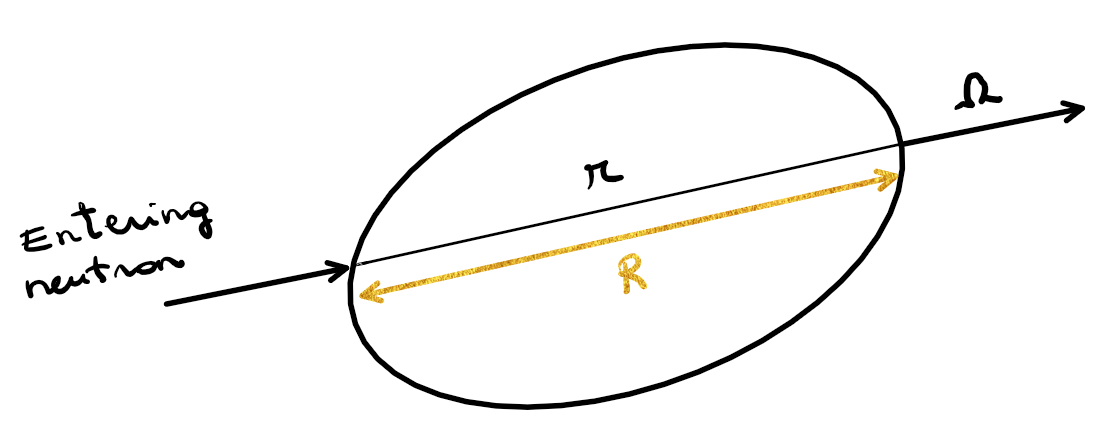
\includegraphics[scale=0.60]{./Figures/P6/dancoff.png} 
  \caption{Geometry for estimating the sticking probability from the escape probability.} 
  \label{fig:dancoff}
\end{figure}

The probability that a neutron, born uniformly along a chord through a pin, will not collide when travelling across a fuel region in a given direction is given as:
\begin{equation*}
    P(\mathbf{\Omega},R) = \frac{1}{R}\int^R_0 \exp\left(-\Sigma_\mathrm{t,f}r\right)\mathrm{d}r = \frac{1}{\Sigma_\mathrm{t,f}R}\left(1- \exp\left(-\Sigma_\mathrm{t,f}R\right)\right)\;\mathrm{,}
\end{equation*}
 while the probability that a neutron, entering from the outside, will collide in the fuel along its way through is:
\begin{equation*}
    G(\mathbf{\Omega},R) = 1-\exp\left(-\Sigma_\mathrm{t,f}R\right)\;\mathrm{,}
\end{equation*}
so we know that:
\begin{equation*}
    G(\mathbf{\Omega},R) = \Sigma_\mathrm{t,f}RP(\mathbf{\Omega},R)\;\mathrm{.}
\end{equation*}
It can be proven that this relationship also holds for the average values:
\begin{equation}
    \langle G\rangle = \Sigma_\mathrm{t,f}\langle R \rangle\langle P\rangle = \Sigma_\mathrm{t,f}\bar{l}\langle P\rangle
\end{equation}
Hence, if we equate $P = \frac{a_\mathrm{B}}{a_\mathrm{B} + \Sigma_\mathrm{t,f}\bar{l}}$, we get
\begin{equation*}
\begin{split}
    P^\mathrm{lattice}_\mathrm{collide} = \frac{\gamma(1-P) + (1-\gamma)\Sigma_\mathrm{t,f}\bar{l}P}{\gamma+(1-\gamma)\Sigma_\mathrm{t,f}\bar{l}P} = \frac{\frac{\gamma\Sigma_\mathrm{t,f}\bar{l}}{a_\mathrm{B} + \Sigma_\mathrm{t,f}\bar{l}} + (1-\gamma)\frac{a_\mathrm{B}\Sigma_\mathrm{t,f}\bar{l}}{a_\mathrm{B}+\Sigma_\mathrm{t,f}\bar{l}}}{\gamma + (1-\gamma)\frac{a_\mathrm{B}\Sigma_\mathrm{t,f}\bar{l}}{a_\mathrm{B}+\Sigma_\mathrm{t,f}\bar{l}}} \\
    = \frac{\gamma\Sigma_\mathrm{t,f}\bar{l} + (1-\gamma)a_\mathrm{B}\Sigma_\mathrm{t,f}\bar{l}}{\gamma a_\mathrm{B} + \gamma \Sigma_\mathrm{t,f}\bar{l} + (1-\gamma)a_\mathrm{B}\Sigma_\mathrm{t,f}\bar{l}} = \frac{\gamma + (1-\gamma) a_\mathrm{B}}{\gamma \frac{a_\mathrm{B}}{\Sigma_\mathrm{t,f}\bar{l}} + \gamma + (1-\gamma)a_\mathrm{B}}\\
    = \frac{1}{\frac{\gamma a_\mathrm{B}}{\Sigma_\mathrm{t,f}\bar{l}\left(\gamma + (1-\gamma)a_\mathrm{B}\right)} + 1} = \frac{\Sigma_\mathrm{t,f}}{\frac{\gamma a_\mathrm{B}\Sigma_\mathrm{e}}{\gamma + a_\mathrm{B}(1-\gamma)} + \Sigma_\mathrm{t,f}} = \frac{\Sigma_\mathrm{t,f}}{\Sigma_\mathrm{t,f} + \frac{\Sigma_\mathrm{e}}{1/a_\mathrm{B} + 1/\gamma - 1}}\;\mathrm{.}
\end{split}
\end{equation*}
This means that the Dancoff correction is another `straightforward' modification to our equivalence theory procedure where our escape cross section takes on a slightly modified form.

The procedure to calculate $\gamma$ can be involved. In modern codes, this is often done with ray tracing, e.g., through the method of characteristics.